\section{Quick start}
\subsection{Overview}

The C3S2 311 Lot 1 - Global Land and Marine Observations Database (GLAMOD) service provides access to in situ surface observations from various climate archives in a common data model.
This document describes the marine component of the service, providing access to surface marine meteorological observations.
This component is currently based on Release 3.0 and Release 3.0.2 of the International Comprehensive Ocean-Atmosphere Data Set (ICOADS, \cite{Freeman2017,Liu2022}) and has been enhanced by: 
\begin{itemize}
\item advanced quality control tests; 
\item enhanced duplicate detection and flagging; 
\item association of instrumental metadata with the observations. 
\end{itemize}
Additional sources, such as from data recovery and digitisation, will be included in future releases.

The observations in ICOADS come from a range of observing platforms, before 1980 these are primarily ships but with an increasing number of measurements made by sensors installed on moored and drifting buoys after this date. 
The ship observations are clustered over the shipping routes prevalent at the time of observation. 
Coverage by drifting buoys tends to be more dispersed but with lower sampling over regions of ocean upwelling. 
Moored buoy data, with the exception of the tropical arrays, tend to be more coastal and concentrated around North America and Europe.

Each meteorological report in ICOADS contains observations of multiple essential climate variables (ECVs, e.g. \cite{Bojinski2014}) made at the same time and location, for example coincident measurements of the air temperature, humidity, wind speed and direction, sea surface temperature and sea level pressure.
From the mid 2000s the record is dominated by reports from drifting buoys but these only report a small subset of the ECVs included in this service, typically only sea level pressure or sea surface temperature.
From 2015 on, this release does not contain drifting buoy data from the ICOADS Release 3.0.2.
A consolidated drifting buoy data record based on additional data sources such as the DBCP Drifting buoys GDAC (\cite{DBCP2022,Coriolis2021}) will be included in future releases.

The reporting frequency ranges from hourly or more frequent in the recent period to daily observations prior to \sim 1860. 
In the intervening period observing frequency ranged from three times per day based on the watches on board ships to 3-hourly or 6-hourly observations.

Several sources of metadata have been used, for the period after \sim 1982 metadata from WMO-No. 47, the "List of Selected, Supplementary and Auxilary Ships" (e.g. \cite{Kent2007}) has been merged with the ship observations.
Some ships observations prior to 1982 have also been merged with the WMO-No. 47 metadata but this is hampered by a lack of ship callsigns within the data before this date.
Additional metadata has been extracted from the ICOADS Supplemental Data (see \cite{Freeman2017}) and documentation available on the ICOADS website.

Apart from the summary information presented in this document, a detailed overview of the data contents for each of the input sources is available in the Marine Data Inventory \\
({C3S2\_D311\_Lot1.2.3.1\_202208\_Marine\_Inventory\_v2}).

\subsection{Essential Climate Variables and observing methods}

Table \ref{tab:ecvs} lists the Essential Climate Variables included in the current release. 
Table \ref{tab:ecvs} also summarises the principle observing methods and changes over time for those ECVs.
Early observations (< 1950s) were typically recorded in whole units, for example whole degrees Celsius or Fahrenheit depending on national practice.
In some cases the data were recorded to higher precisions but truncated or rounded when digitised (e.g. \cite{Chan2019}) or shared operationally. 
This rounding for operational data streams persisted until the 1980s (e.g. \cite{Willett2008}).
Later observations were typically recorded and shared with precisions of tenths or higher.
As part of the processing to create ICOADS (and earlier datasets) the observations were converted to standardised units (°C for temperatures, hPa for pressure and m/s for speeds) and uniform resolution, typically to one or two decimal places.
These have been further processed as part of the GLAMOD service and fully converted to S.I. units.
Where recorded, the originally reported value and units will be made available.
There are known issues with the marine meteorological observations, these are discussed further in Section \ref{data_sources}.
No corrections or adjustments have been applied as part of this service, instead the user is directed to the literature identified within Section \ref{data_sources}.

\begin{table}[h]
\centering
\caption{Essential Climate Variables included in the GLAMOD service}
\label{tab:ecvs}
% \begin{center}
%\begin{tabular}{|p{0.2\linewidth}|p{0.25\linewidth}|p{0.5\linewidth}|}
\begin{tabular}{|p{0.25\linewidth}|p{0.65\linewidth}|}
\hline
% Variable & Typical precision & Description \\ 
\bfseries Variable & \bfseries Description \\ 
\hline
%Air temperature & Either tenths or whole °C or Fahrenheit & Air temperature at observation height, ranging from 4 - 5 m in the 19th century to over 30 m for the modern period. Typically measured using liquid in glass thermometers (mercury or alcohol) but with a transition to electronic sensors over the past 30 years.\\
Air temperature & Air temperature at observation height, ranging from 4 - 5 m in the 19th century to over 30 m for the modern period. Typically measured using liquid in glass thermometers (mercury or alcohol) but with a transition to electronic sensors over the past 30 years.\\
\hline
%Dew point temperature & Either tenths or whole °C or Fahrenheit & Dew point temperature at observation height, usually the same as for air temperature. Typically calculated from wet and dry bulb thermometers housed in marine screens or whirling psychrometers. Over the past 30 years there has been a transition to electronic sensors measuring relative humidity.\\
Dew point temperature & Dew point temperature at observation height, usually the same as for air temperature. Typically calculated from wet and dry bulb thermometers housed in marine screens or whirling psychrometers. Over the past 30 years there has been a transition to electronic sensors measuring relative humidity.\\
\hline
%Sea surface temperature & Either tenths or whole °C or Fahrenheit. Hundredths of °C for some sources & Water temperature at the sea surface measured using a variety of methods. Typically bucket measurements pre 1950 but with a transition to engine intake measurements beginning around 1900. Dominated by drifting buoy observations after ~ 2003.\\
Sea surface temperature & Water temperature near the sea surface measured using a variety of methods.
This temperature does not represent the skin sea surface temperature. Depending on the method, the temperature is measured in depths from a few centimeters to several meters.
Typically bucket measurements pre 1950 but with a transition to engine intake measurements beginning around 1900. Dominated by drifting buoy observations after \sim 2003.\\
\hline
%Sea level pressure & Typically tenths hPa & Atmospheric pressure reduced to sea level and corrected for temperature where appropriate. Methods range from mercury barometers in the 19th Century, through aneroid barometers to electronic sensors.\\
Sea level pressure & Atmospheric pressure reduced to sea level and corrected for temperature where appropriate. Methods range from mercury barometers in the 19th Century, through aneroid barometers to electronic sensors. It should be noted that the sea level reduction and temperature corrections are applied at the time of observation.\\
\hline
%Wind speed & Beaufort Force, whole knots and m/s. Tenths units in recent periods& Wind speed at observation height. As with air temperature and dew point temperature the observation height has varied from < 10 m in the early record to more than 30 m for recent years. Methods include visual wind speed estimation for the early record transitioning to mechanical sensors (cup/propellor anemometers) and electronic sensors (sonic anemometers). Instrumental observations corrected for ship speed and course (not applicable for visual estimation).\\
Wind speed & Wind speed at observation height. As with air temperature and dew point temperature, the observation height has varied from < 10 m in the early record to more than 30 m for recent years. Methods include visual wind speed estimation for the early record transitioning to mechanical sensors (cup/propellor anemometers) and electronic sensors (sonic anemometers). Instrumental observations corrected for ship speed and course (not applicable for visual estimation).\\
\hline
%Wind Direction & Compass point (early record) to 10s of degrees and higher in the recent period & See wind speed.\\
Wind Direction & See wind speed.\\
\hline
\end{tabular}
%\end{center}
\end{table}

\subsection{Coverage}
The temporal coverage of the data available in the current release spans the period \datatimerange{}, Figure \ref{fig:ecv_ts1} shows the coverage per ECV. 
Before the Brussels International Maritime Conference of 1853 the most common ECVs to be reported were: air temperature; wind speed / force and direction; and sea level pressure, with typically \sim 100 - 200 observations per month. 
A small number of sea surface temperature and humidity observations are available (< 100).
Following the Brussels conference there is a large increase in number of observations to O(10,000) per month for all parameters excluding dew point temperature. 
Dew point observations only reach 10,000 per month on a routine basis around the time of the First World War.
For all parameters, the number of observations increases over time to around 100,000 per month in the 1960s and remains at this level until the 1990s.
From the mid 1990's there is a large increase in the number of sea level pressure and sea surface temperature observations from drifting buoys.
From 2015 on, drifting buoys are not included in this release, resulting in a drop in the number of sea surface temperature and sea level observations.

\begin{figure}[h]
\centering
%\begin{center}
    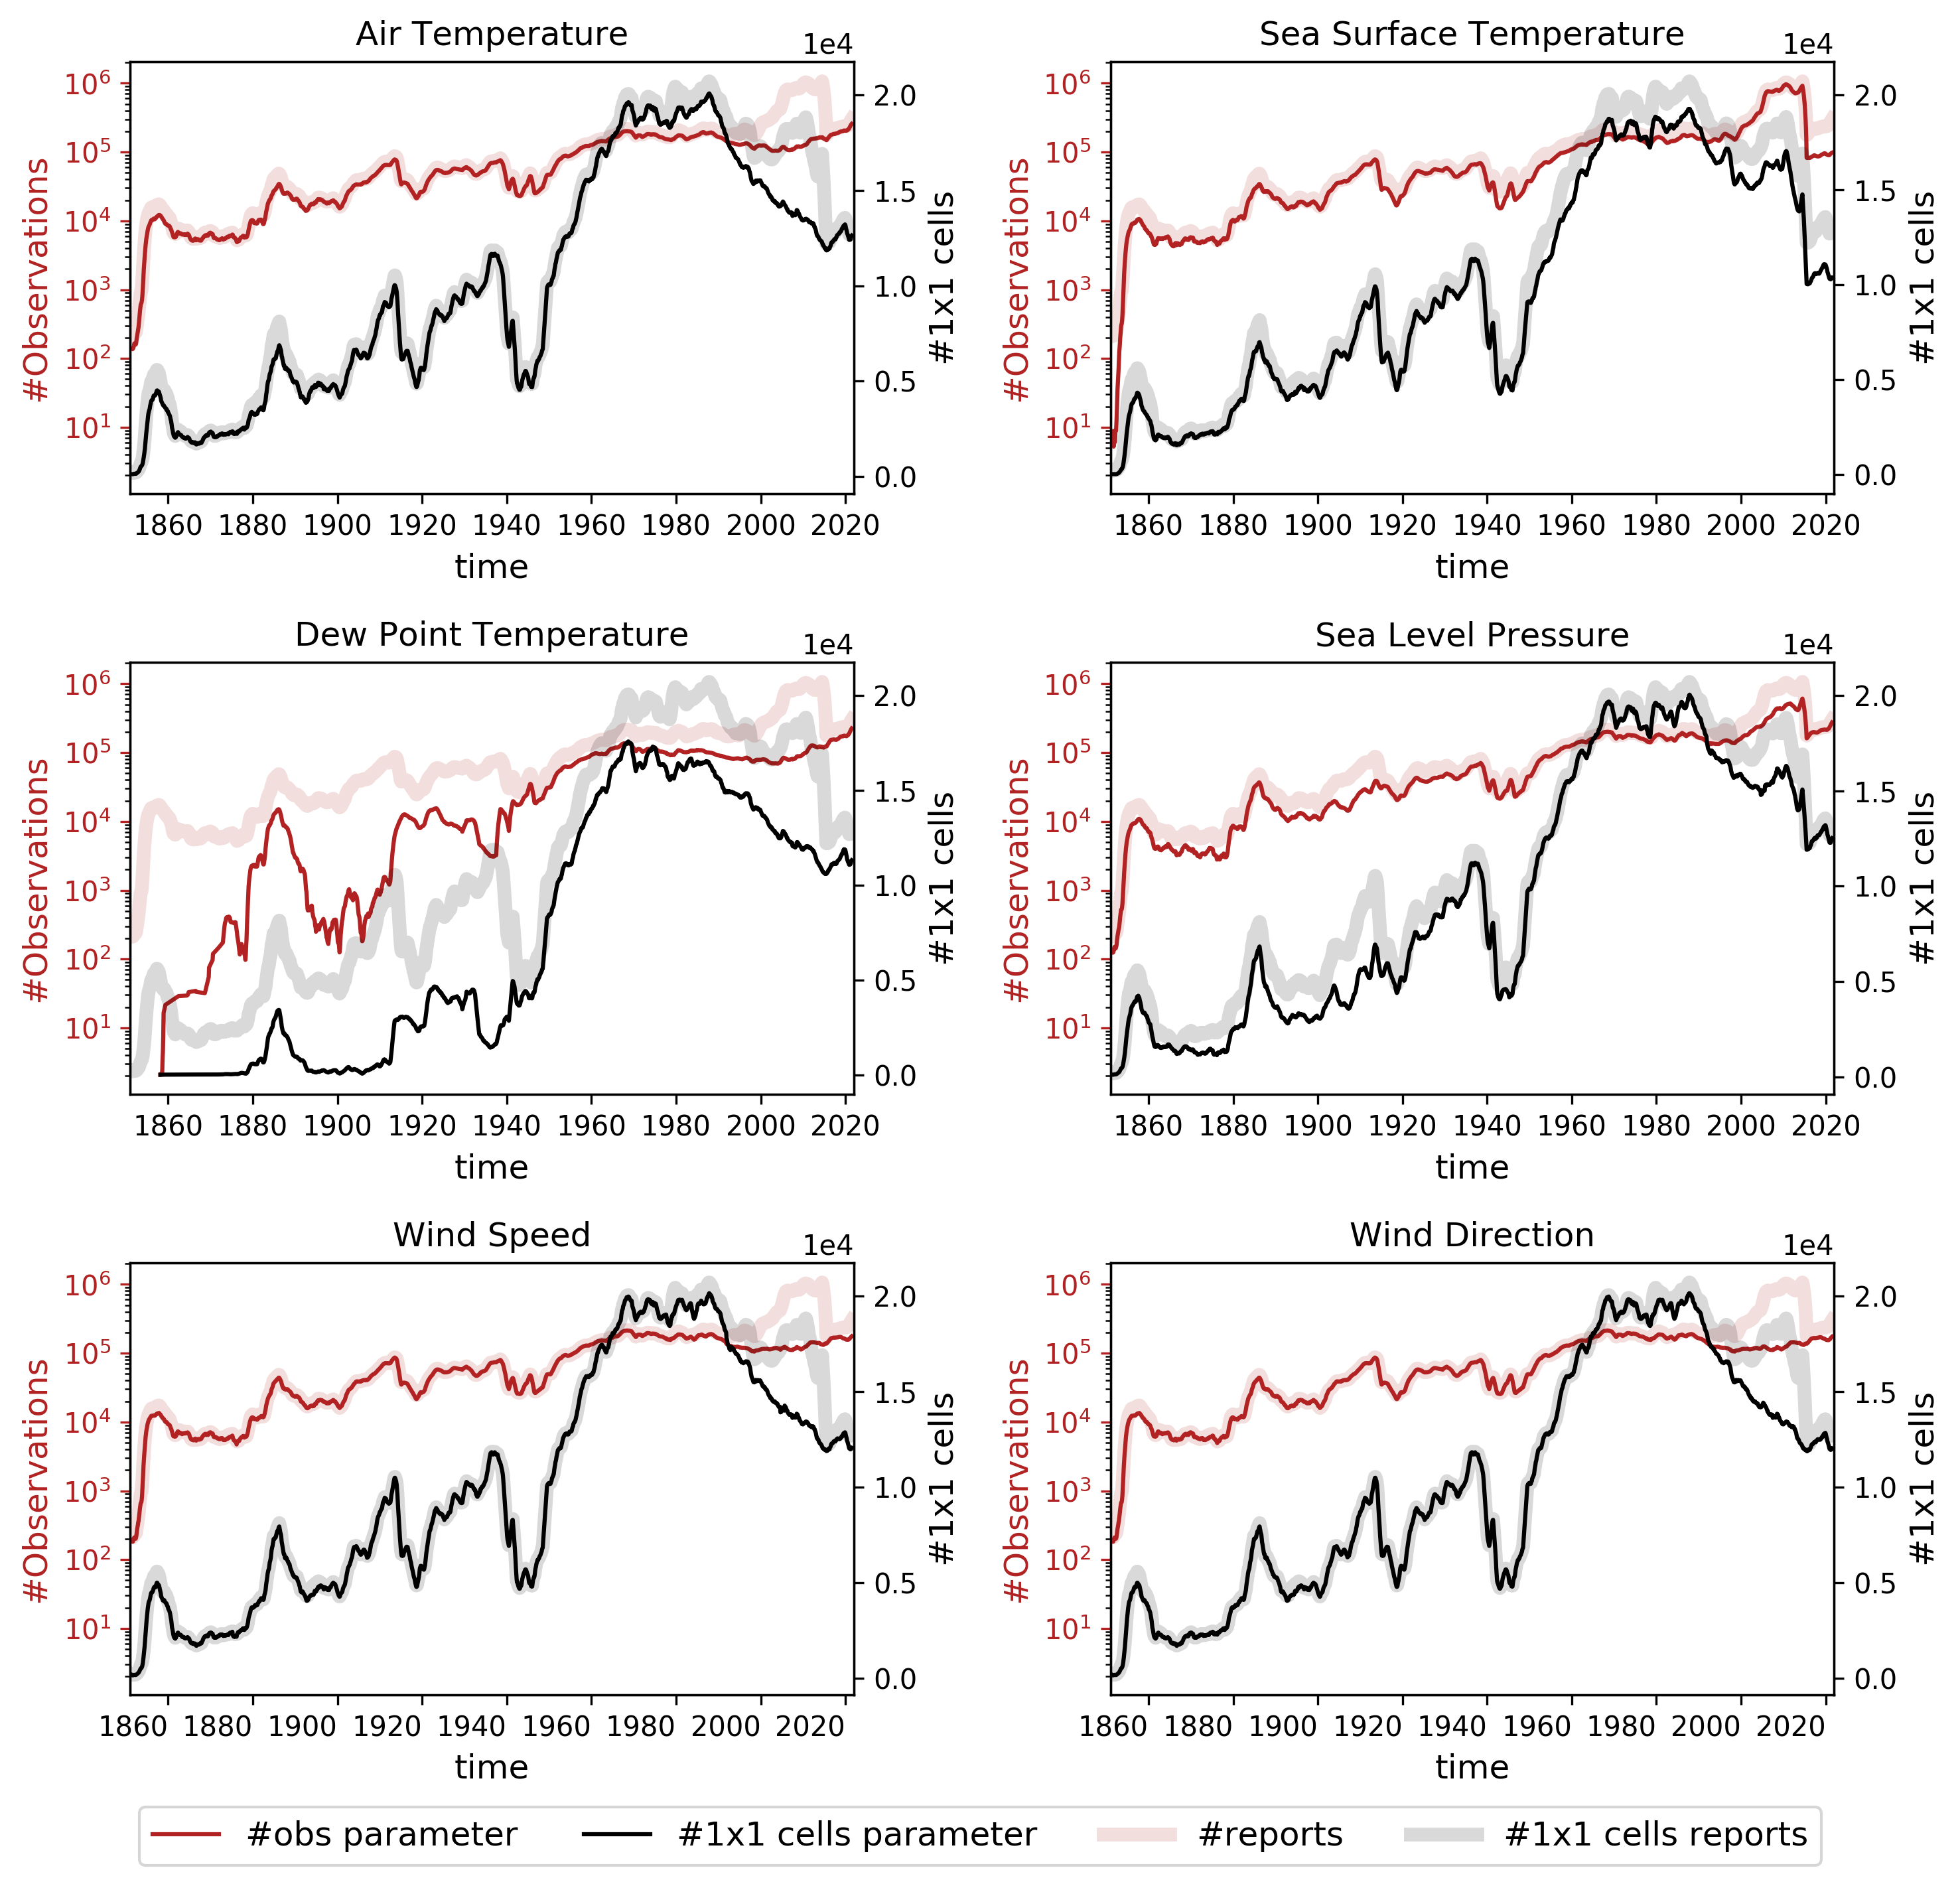
\includegraphics[width=0.75\textwidth]{resources/ecv_coverage_ts_grid.png}
    \caption{Availability of ECVs listed in Table \ref{tab:ecvs} by time. Both the number of observations (red) and number of grid cells (black) with data are shown. Note log scale for the number of observations.\\}.
    \label{fig:ecv_ts1}
%\end{center}
\end{figure}

Figure \ref{fig:nreports-map1} shows the total number of reports and total number of months per 1x1 degree grid cell, however over the period \datatimerange{} there have been major changes to the spatial sampling.
Early in the record there were typically a few hundred 1x1 degree grid cells with data per month (see Figure \ref{fig:ecv_ts1}).
These tended to be concentrated in the Atlantic Ocean and around the southern capes to the Indian and Pacific Oceans.
With the opening of the Suez and then Panama canals the major shipping routes changed, with less shipping transiting the capes and a greater proportion transiting the Mediterranean and Caribbean seas to reach the Indian and Pacific oceans.
Spatial coverage reached a peak between the 1960s and 1990s but declined sharply after 1990.
The number of grid cells dropped from around 20,000 to around 10,000 - 12,000 by 2020 for the majority of parameters. 
The contrast between the stable number of observations and decreasing spatial coverage (contrasting red and black lines in Figure \ref{fig:ecv_ts1}) is due to the change in reporting frequency from 6 hourly to 3 or 1 hourly and greater over the past 30 years, increasing the temporal sampling at the cost of spatial sampling.
Sea level pressure and sea surface temperature experience a much smaller marked decline in spatial coverage due to the contribution of drifting buoys.

It should be noted that observations for the period 1784 - 1850 were also processed as part of this release but due to missing time information and the sparseness of the data neither the quality control nor duplicate detection software has been run for this period. These data are available by selecting the "all data" option when downloading but should be used with caution.


\begin{figure}[h]
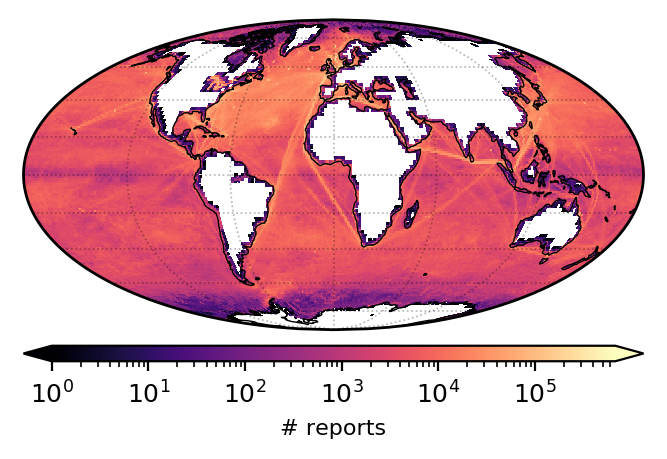
\includegraphics{resources/header-reports-map-optimal.png}
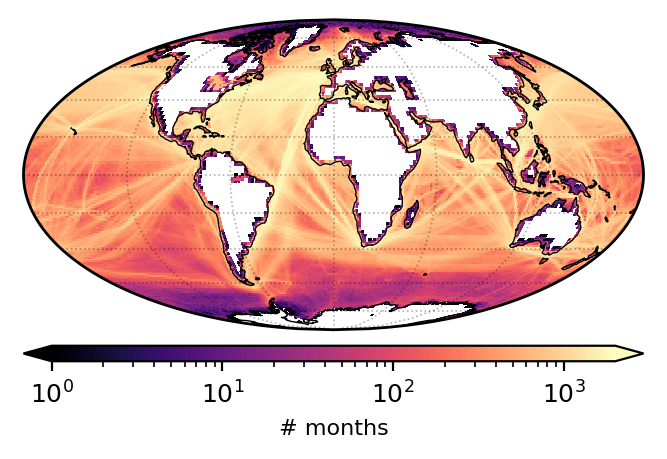
\includegraphics{resources/header-months-map-optimal.png}
\caption{Spatio-temporal distribution of marine data holdings \datatimerange{}. Left: number of reports per grid cell; right: number of months with at least 1 report. Grid size is 1x1. Note logarithmic colour scale. Only reports passing the report level QC checks flag have been included.\\}
\label{fig:nreports-map1}
\end{figure}

\newpage
\subsection{Data access}
The data can be downloaded and accessed via the Copernicus Climate Change Service (C3S) Climate Data Store (CDS):
\begin{center}
\sloppy\url{https://cds.climate.copernicus.eu/cdsapp#!/dataset/insitu-observations-surface-marine?tab=form}.
 \end{center}
The page has 3 tabs, the Overview tab presents an overview of the marine data and provides details on the data description, main and related variables available, contact email and links to licence/data policy statements. 
The Documentation tab provides links to PDF’s of the Marine Product User Guide, Marine data inventories, Common Data Model specifications and a link to the Data Deposit Server webpage. The Download Data tab provides 6 sections that need to be completed in order to download data. The first selects one or more variables (Figure \ref{fig:cds_variable}) from the available ECVs (Table \ref{tab:ecvs}). The second selects the level of quality control to apply, selecting either those that have passed all stages of quality control or all observations (Figure \ref{fig:cds_qc}). The next three select the time period  by selecting the year (Figure \ref{fig:cds_year}), month (Figure \ref{fig:cds_month}) and day (Figure \ref{fig:cds_day}). The final selection selects the region, specifying either all data (global) or selecting observations within a bounding box (Figure \ref{fig:cds_area}).

Data can additionally be downloaded using the CDS Python API. Selecting the \texttt{Show API request} button reveals the API commands to use for the given selection (Figure \ref{fig:cds_api}). More information can be found at:
\begin{center}
\url{https://cds.climate.copernicus.eu/api-how-to}
\end{center}

\FloatBarrier
\begin{figure}[h]
\centering
%\begin{center}
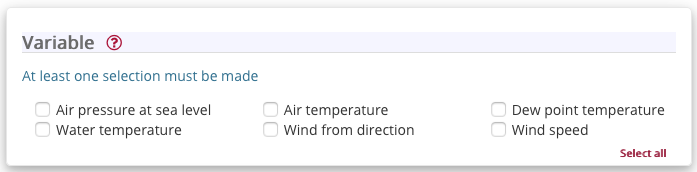
\includegraphics[width=0.75\textwidth]{resources/cds_variable_select.png}
\caption{Selection box for variable selection on the Global Land And Marine Observations Database download page on the CDS. It should be noted that "water temperature" is used in the data model to include river, lake and sea surface temperature.\\}
\label{fig:cds_variable}
%\end{center}
\end{figure}


\begin{figure}
\centering
%\begin{center}
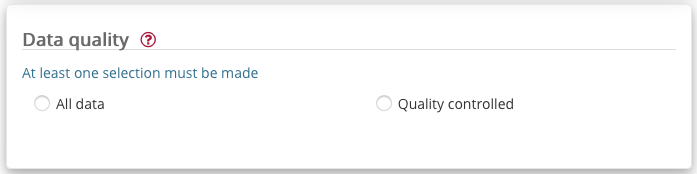
\includegraphics[width=0.75\textwidth]{resources/cds_qc_select.png}
\caption{Selection box for quality status on the Global Land And Marine Observations Database download page on the CDS.\\}
\label{fig:cds_qc}
%\end{center}
\end{figure}

\begin{figure}
\centering
%\begin{center}
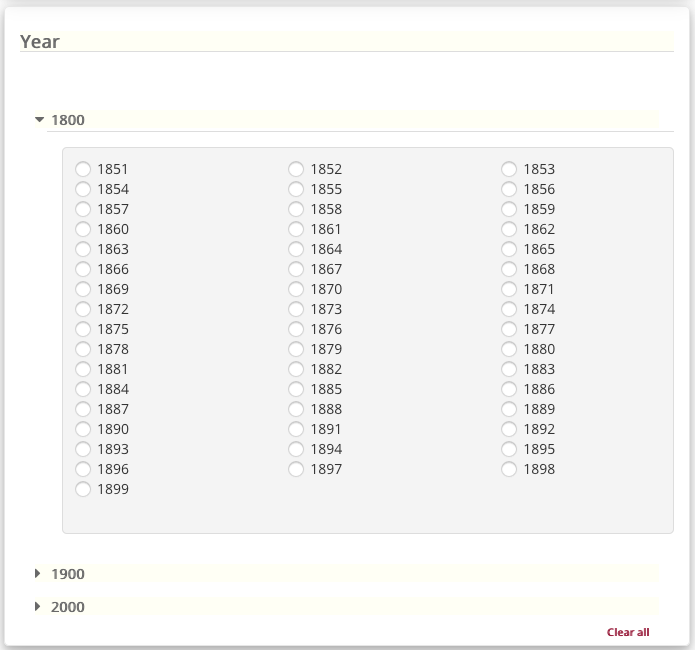
\includegraphics[width=0.75\textwidth]{resources/cds_year_select.png}
\caption{Selection box for selecting year on the Global Land And Marine Observations Database download page on the CDS.\\}
\label{fig:cds_year}
%\end{center}
\end{figure}

\begin{figure}
\centering
%\begin{center}
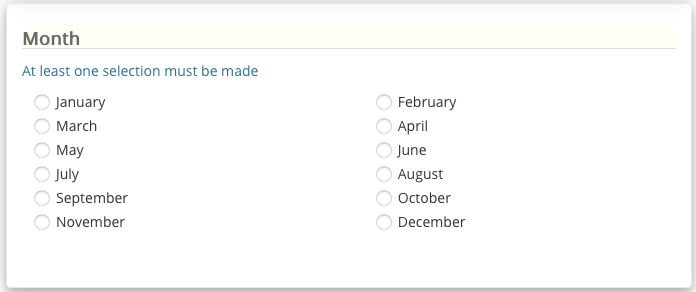
\includegraphics[width=0.75\textwidth]{resources/cds_month_select.png}
\caption{Selection box for selecting month on the Global Land And Marine Observations Database download page on the CDS.\\}
\label{fig:cds_month}
%\end{center}
\end{figure}

\begin{figure}
\centering
%\begin{center}
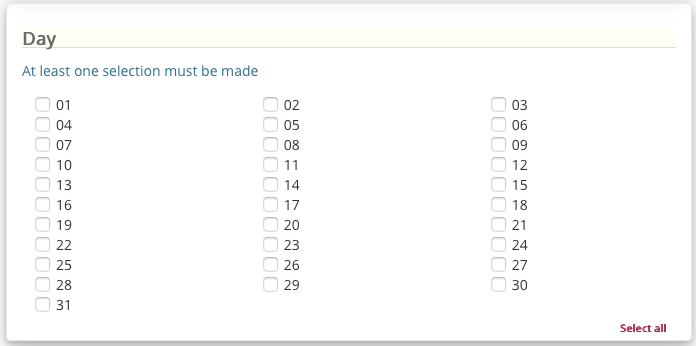
\includegraphics[width=0.75\textwidth]{resources/cds_day_select.png}
\caption{Selection box for selecting day on the Global Land And Marine Observations Database download page on the CDS.\\}
\label{fig:cds_day}
%\end{center}
\end{figure}

\begin{figure}
\centering
%\begin{center}
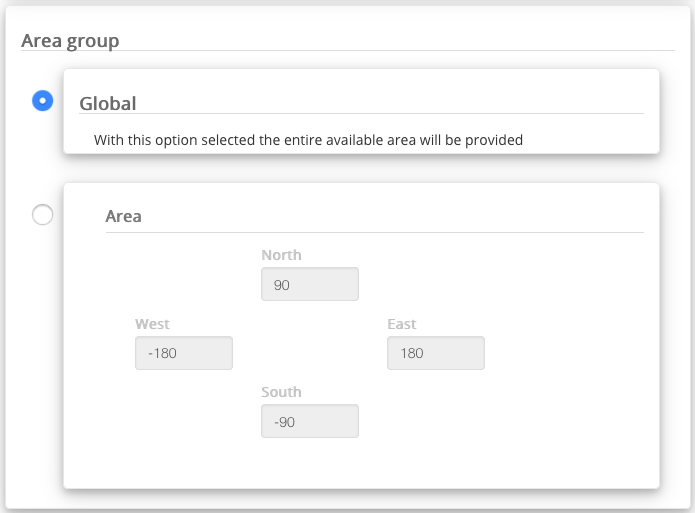
\includegraphics[width=0.75\textwidth]{resources/cds_area_select.png}
\caption{Selection box for selecting area on the Global Land And Marine Observations Database download page on the CDS.\\}
\label{fig:cds_area}
%\end{center}
\end{figure}

\begin{figure}
\centering
%\begin{center}
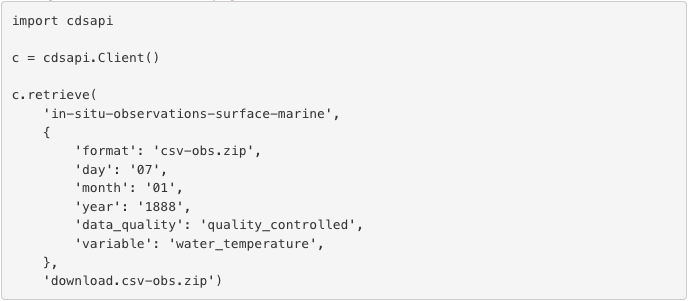
\includegraphics[width=0.75\textwidth]{resources/cds_api_request.png}
\caption{Example API request to download data from the Global Land And Marine Observations Database.\\}
\label{fig:cds_api}
%\end{center}
\end{figure}

\FloatBarrier
\subsection{Data model}
\label{subsection:data_model}
Data from the Climate Data Store are returned in delimited text files (.csv), with 19 columns per row and one observed value per row. 
The columns are listed in table \ref{tab:cdm_lite} together with a brief description.  
The date and time of the observation is given by the \code{date\_time} column, with the value returned as a string of the format \code{YYYY-MM-DD hh:mm:ss}. 
All data are returned in the UTC time zone.
The location of the observation is given by the \code{latitude} and \code{longitude} columns in the WGS84 / EPSG4326 coordinate reference system. 
The variable being reported / observed is given by the \code{observed\_variable} column, the units by the \code{units} column and the observed value by the \code{observation\_value} column. 
The remaining columns provide further contextual information for the observations, such platform type and station identifiers etc. 
%A number of the columns are enumerated using code tables, indicated by the text \code{(coded)} in the Kind column of Table \ref{tab:cdm_lite}.
%These code tables are reproduced in tables \ref{tab:report_type} to \ref{tab:licence} but with only those values used in the marine data listed.

\csvreader[
  longtable=|p{0.25\linewidth}|p{0.2\linewidth}|p{0.45\linewidth}|,
  table head=\caption{Data model.\label{tab:cdm_lite}}\\
    \hline\bfseries Field &\bfseries Kind &\bfseries Description \\ \hline\endfirsthead
    \multicolumn{3}{c} {{\tablename\ \thetable{} -- continued from previous page}} \\ 
    \hline\bfseries Field &\bfseries Kind &\bfseries Description \\ \hline\endhead
    \hline\endfoot,    
    separator=semicolon,
    late after line=\\ \hline
]{./data_model/cdm_lite.csv}{1=\Field,2=\Kind,3=\Description}{\Field & \Kind & \Description }
